\documentclass[xcolor={dvipsnames}]{beamer}

\usetheme{Malmoe}
\usecolortheme{seagull}
\usepackage[]{natbib}
\usepackage{textpos}
\usepackage{amsmath, amssymb, bm}
\usepackage{multirow}
\usepackage{framed}
\usepackage{schemata}
\setbeamertemplate{navigation symbols}{}
\usepackage[english]{babel}
\usepackage{animate}
\usepackage{graphics}
\usepackage{fontawesome}


\definecolor{lightblue}{rgb}{0.145,0.6666,1} % Defines the color used for content box headers
\definecolor{Red}{rgb}{0.9,0.15,0}
\definecolor{Blue}{RGB}{55,126,184}
\definecolor{Green}{RGB}{77,175,74}
\definecolor{White}{RGB}{255,255,255}
\definecolor{Lightgray}{rgb}{0.86,0.86,0.86}

\setbeamertemplate{footline}
{
	\leavevmode%
	\hbox{%
		\begin{beamercolorbox}[wd=.50\paperwidth,ht=2.25ex,dp=1ex,center]{author in head/foot}%
			\usebeamerfont{author in head/foot}\insertshortauthor%% \beamer@ifempty{\insertshortinstitute}{}{(\insertshortinstitute)}
		\end{beamercolorbox}%
%		\hskip2pt%
		\begin{beamercolorbox}[wd=.50\paperwidth,ht=2.25ex,dp=1ex,center]{title in head/foot}%
			\usebeamerfont{title in head/foot}\insertshorttitle~~~~~~~~~~~~~~~~~~~~~~~~~~\insertframenumber
		\end{beamercolorbox}%
	}%
	\vskip0pt%
}
\makeatother

\title[Lifespan inequality in Denmark]{
	\small{\textsl{EPC 2018}}\\$\,$\\$\,$}

\subtitle{\large{\textsc{Potential gains in life expectancy by reducing inequality of lifespans in Denmark}}\\$\,$\\}


\author[EPC 2018. Aburto et al 2018]
{
	\vspace{-0.5cm}
	\texorpdfstring{
		\begin{columns}
			\column{.9\linewidth}
			\centering
			\normalsize{JM Aburto, M Wensink, A van Raalte, R Lindahl-Jacobsen}\\
			$\,$\\
			
\includegraphics[scale=0.2]{Figures/SDU_Logo}     
		\end{columns}
	}
	{Jos\'{e} Manuel Aburto}
}

\date[]{ April 2018}

\beamertemplatenavigationsymbolsempty
\begin{document}


\begin{frame}[plain]
	\titlepage
\end{frame}
%%%%%%%%%%%%%%%%%%%%%%%%%%%%%%%%%%%%%%%%%%%%%%%%%%%%%%%%%%%%%%%%%%%%%%%%%
%%%%%%%%%%%%%%%%%%%%%%%%%%%%%%%%%%%%%%%%%%%%%%%%%%%%%%%%%%%%%%%%%%%%%%%%%
\section{Introduction}

%%%%%%%%%%%%%%%%%%%%%%%%%%%%%%%%%%%%%%%%%%%%%%%%%%%%%%%%%%%%%%%%%%%%%%%%%
\begin{frame}
\Large{
		\begin{itemize}
		
		\item<1-> \textbf{Highest} mortality from all neoplasms in Europe.
		
		\item<2-> Females $\longrightarrow$ \textbf{highest} lung cancer mortality rates in Europe.
		
        \item<3-> Males have \textbf{higher smoking-related mortality} than Swedish males.

        \item<4-> Females born in 1919-1939 $\longrightarrow$ \textbf{high levels of smoking and alcohol consumption}.
		
		\end{itemize}
		
}

\end{frame}


\begin{frame}\frametitle{As a result}

\Large{
		\begin{itemize}
		    \item Danish life expectancy \textbf{stagnated} in 1975-1995 ($\backsim $77y)
		\end{itemize}
		
		\pause
				\begin{center}
		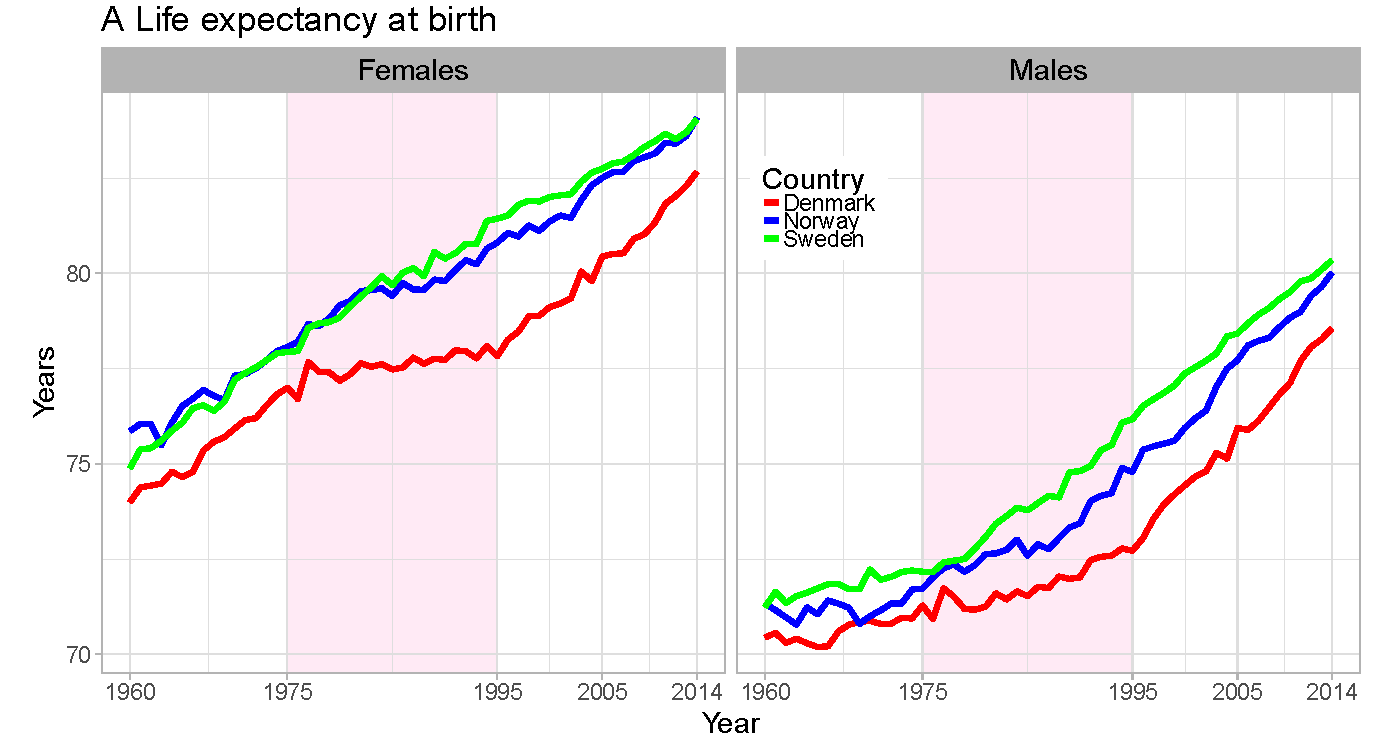
\includegraphics[scale=.45]{Figures/Figure_0}
				\end{center}
				

}
\end{frame}

\begin{frame}\frametitle{Motivation}
\large{
		\begin{itemize}
		
		\item \textbf{Lifespan inequality} increasingly recognized as public health goal.\pause
		
		\item \textbf{Effect of smoking-related and overall cancer} on lifespan inequality is unknown. \pause
		
		\item \textbf{Shared} history, culture and similarities in healthcare systems with Sweden and Norway. 
		\end{itemize}
		\pause
		
		\begin{center}
		\Large{\textbf{What does Denmark need to close the gap in $e_0$
		through lifespan inequality?}}
		\end{center}
		
}

\end{frame}




\begin{frame}\frametitle{Why lifespan inequality?}
\Large{
		\begin{itemize}
		
		\item<1-> \textbf{Complements} life expectancy (mean) with variation of lifespans.

		\item<2-> \textbf{Heterogeneity} in age at death at the \textbf{macro level}.
		
		\item<3-> \textbf{Uncertainty} in the timing of death at the \textbf{micro level}
		
		\item<4-> We make \textbf{decisions} based on both.
						
		\end{itemize}

}
\end{frame}


\begin{frame}\frametitle{Why lifespan inequality?}

				\begin{center}
		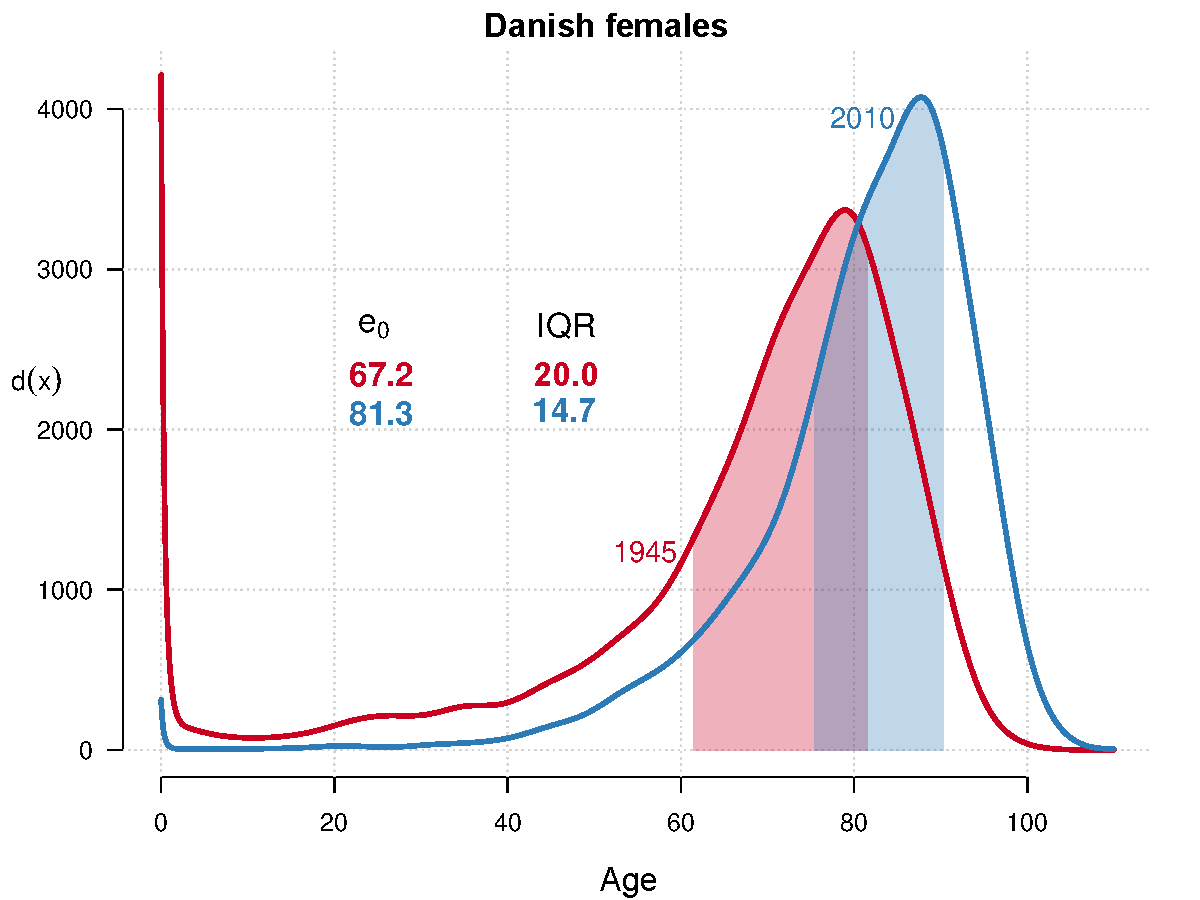
\includegraphics[scale=.48]{Figures/Danish_distribution}
				\end{center}
				
\end{frame}



\section{Methods}


\begin{frame}\frametitle{Data}
\Large{
		\begin{itemize}
		
		\item \textbf{Period lifetables} from HMD for Denmark, Sweden and Norway from 1960-2014.

		\item \textbf{Cause of death} data from WHO database.
		
		\end{itemize}

}
\end{frame}

\begin{frame}\frametitle{Classification of deaths}
\Large{

		\begin{enumerate}
		
		
\color{blue} 		\item Cancer sensitive to smoking

\color{green}		\item Cancer non-sensitive to smoking
		
\color{ForestGreen}	\item Cardiovascular conditions
		
\color{orange}		\item Non-infectious respiratory diseases
		
\color{Orange}	    \item Infectious respiratory diseases

\color{Red}	       \item External causes
		
\color{gray}       \item Rest.

		
		\end{enumerate}			

}
\end{frame}




%\begin{frame}\frametitle{Sensitivity}
%
%				\begin{center}
%		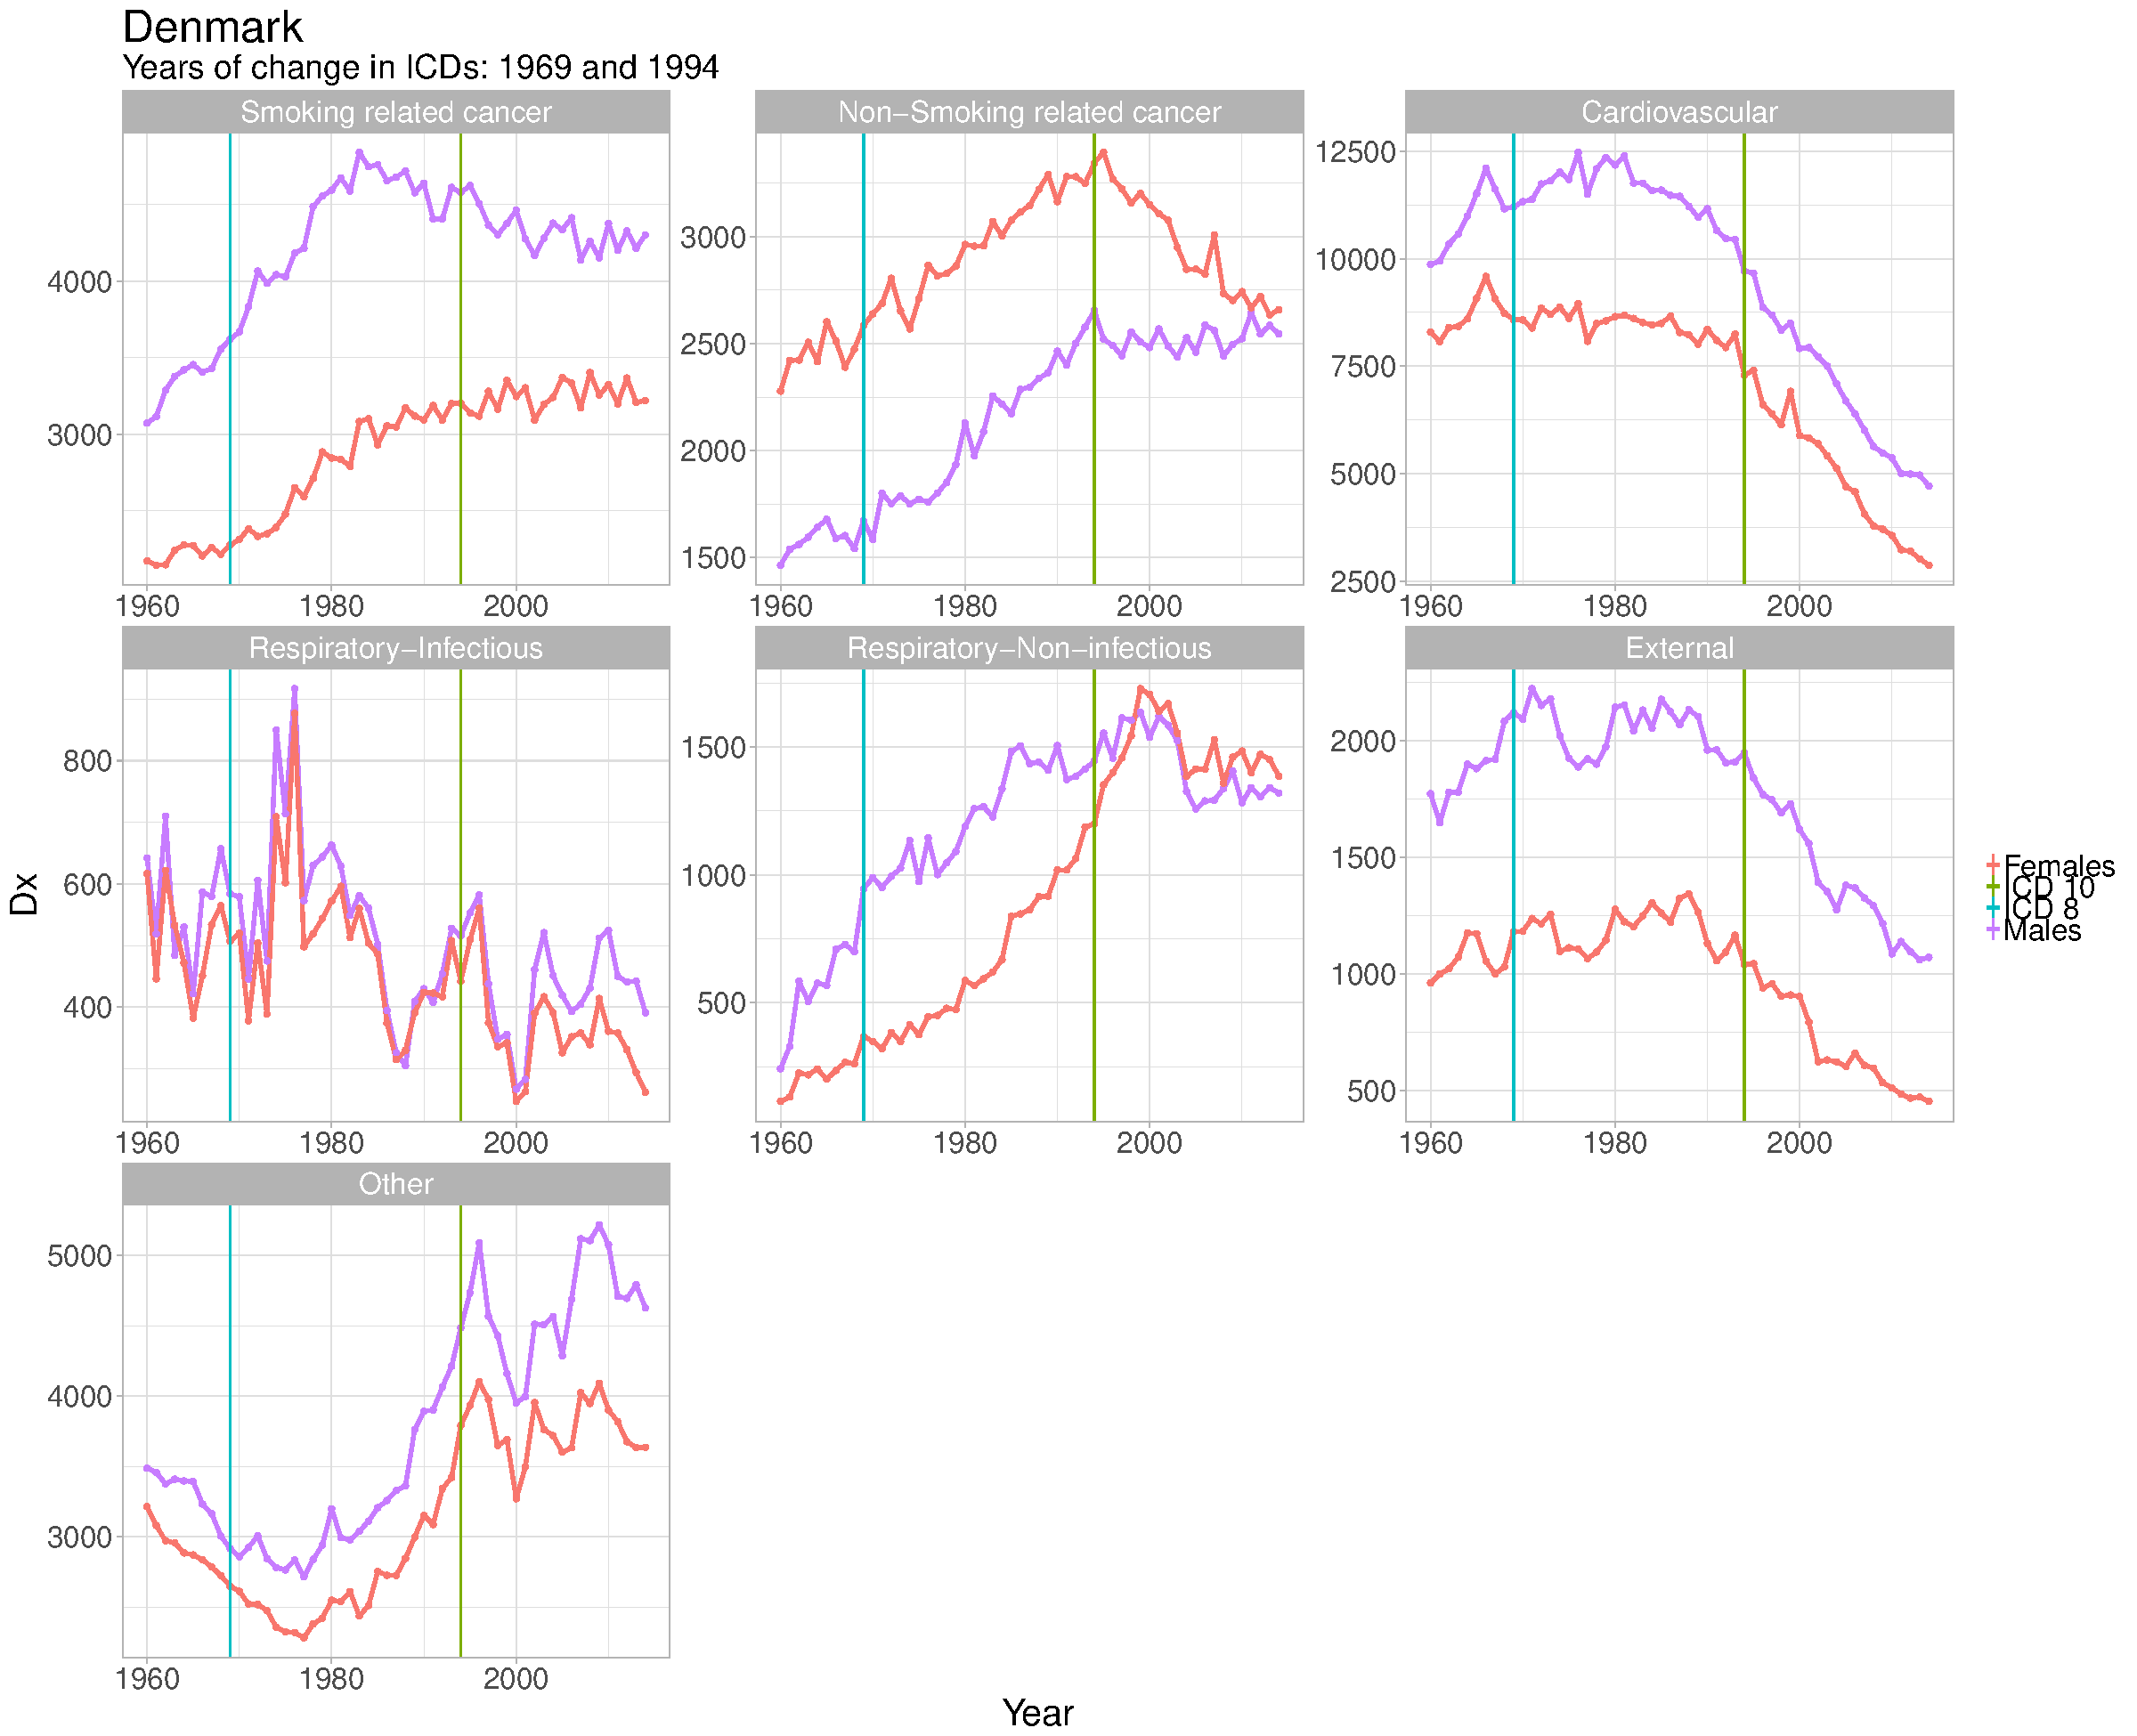
\includegraphics[scale=.22]{Figures/Sensitivity}
%				\end{center}
%				end{frame}



\begin{frame}
\Large{
\textbf{Indicator: Coefficient of variation}
\pause
\begin{itemize}
\item Standard deviation divided by the mean
\begin{equation*}
\frac{\sigma}{e_0}
\end{equation*}
\item Captures the \textbf{dimensionless} of the shape of aging.
\pause
\item \textbf{Easy} to interpret.
\pause
\item Allows to separate ages and causes that \textbf{decrease} from those that \textbf{increase} inequality.
\end{itemize}

}
\end{frame}


\section{Results}



\begin{frame}
\hspace*{-.4in}
		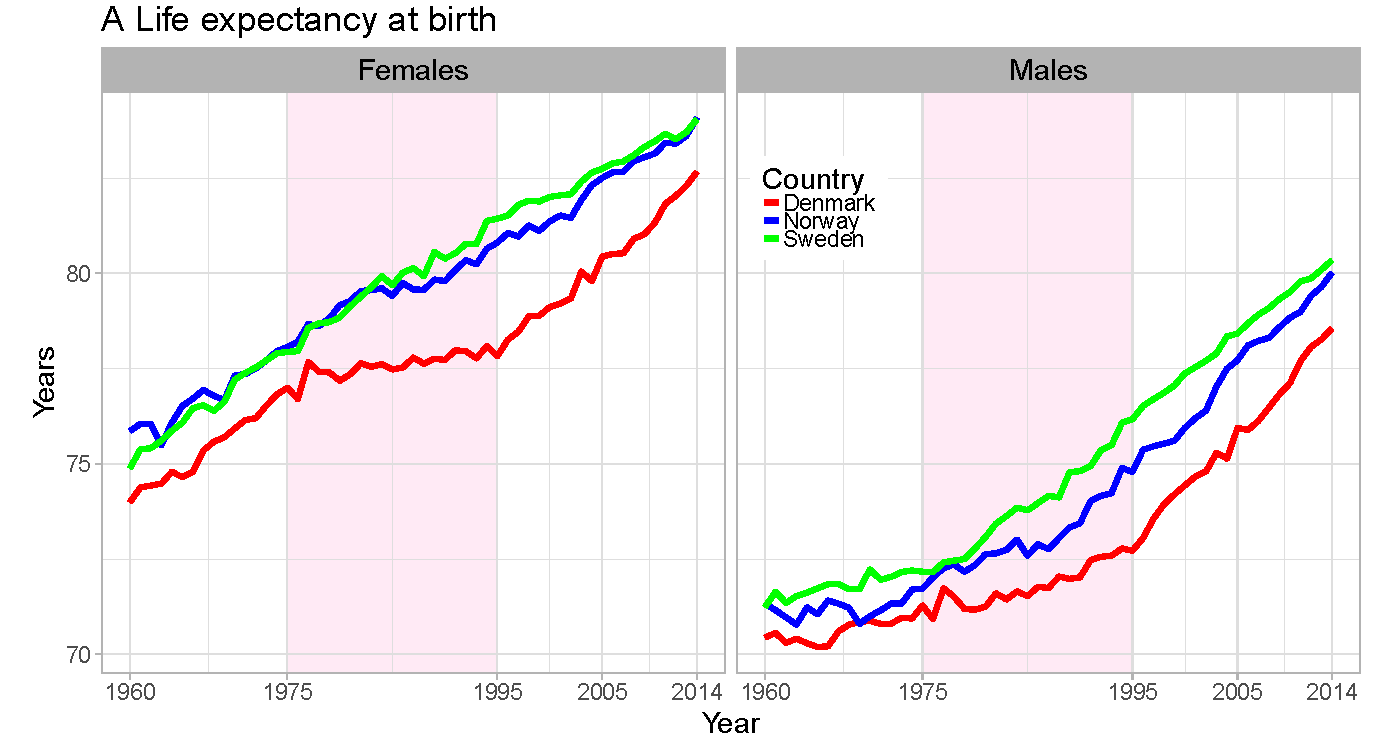
\includegraphics[scale=.53]{Figures/Figure_0}	
\end{frame}


\begin{frame}
\hspace*{-.35in}
		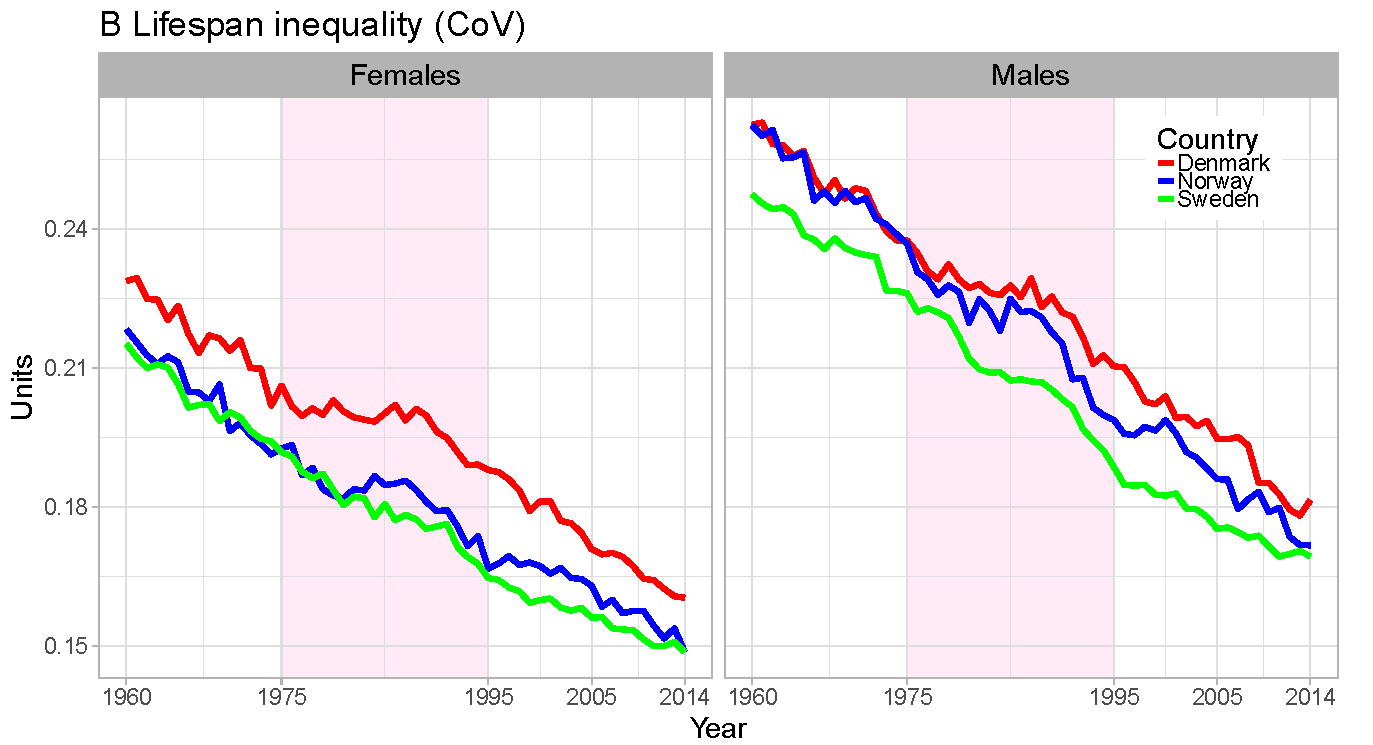
\includegraphics[scale=.53]{Figures/Figure_1_2}	
\end{frame}

\begin{frame}
\hspace*{-.4in}
		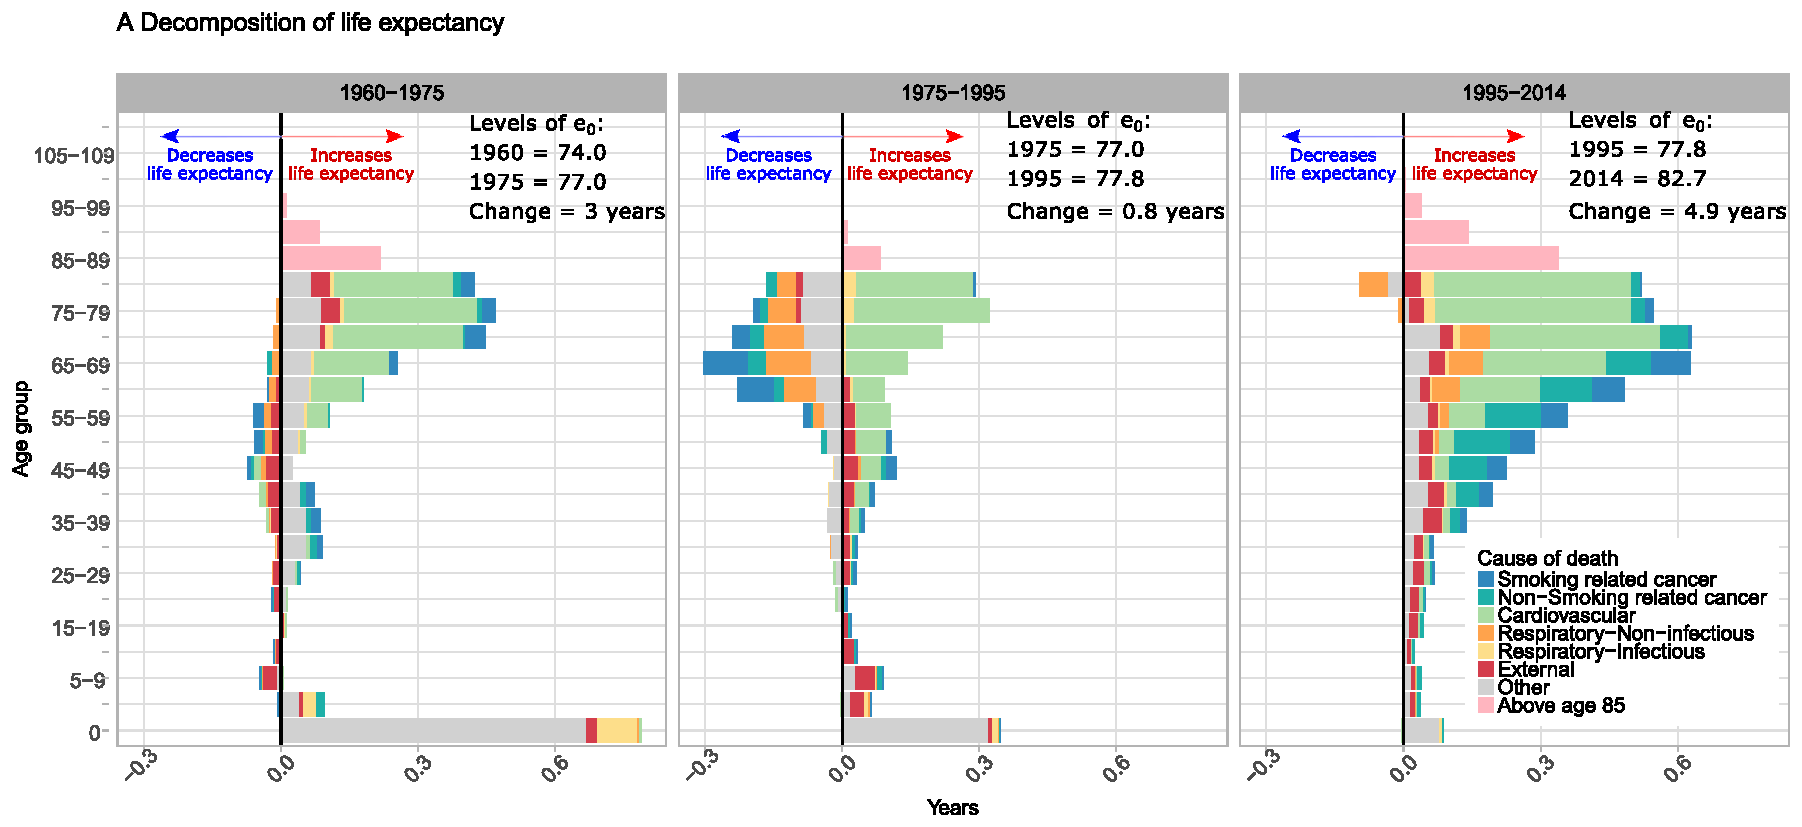
\includegraphics[scale=.41]{Figures/Figure_2_1}	
\end{frame}


\begin{frame}
\hspace*{-.4in}
		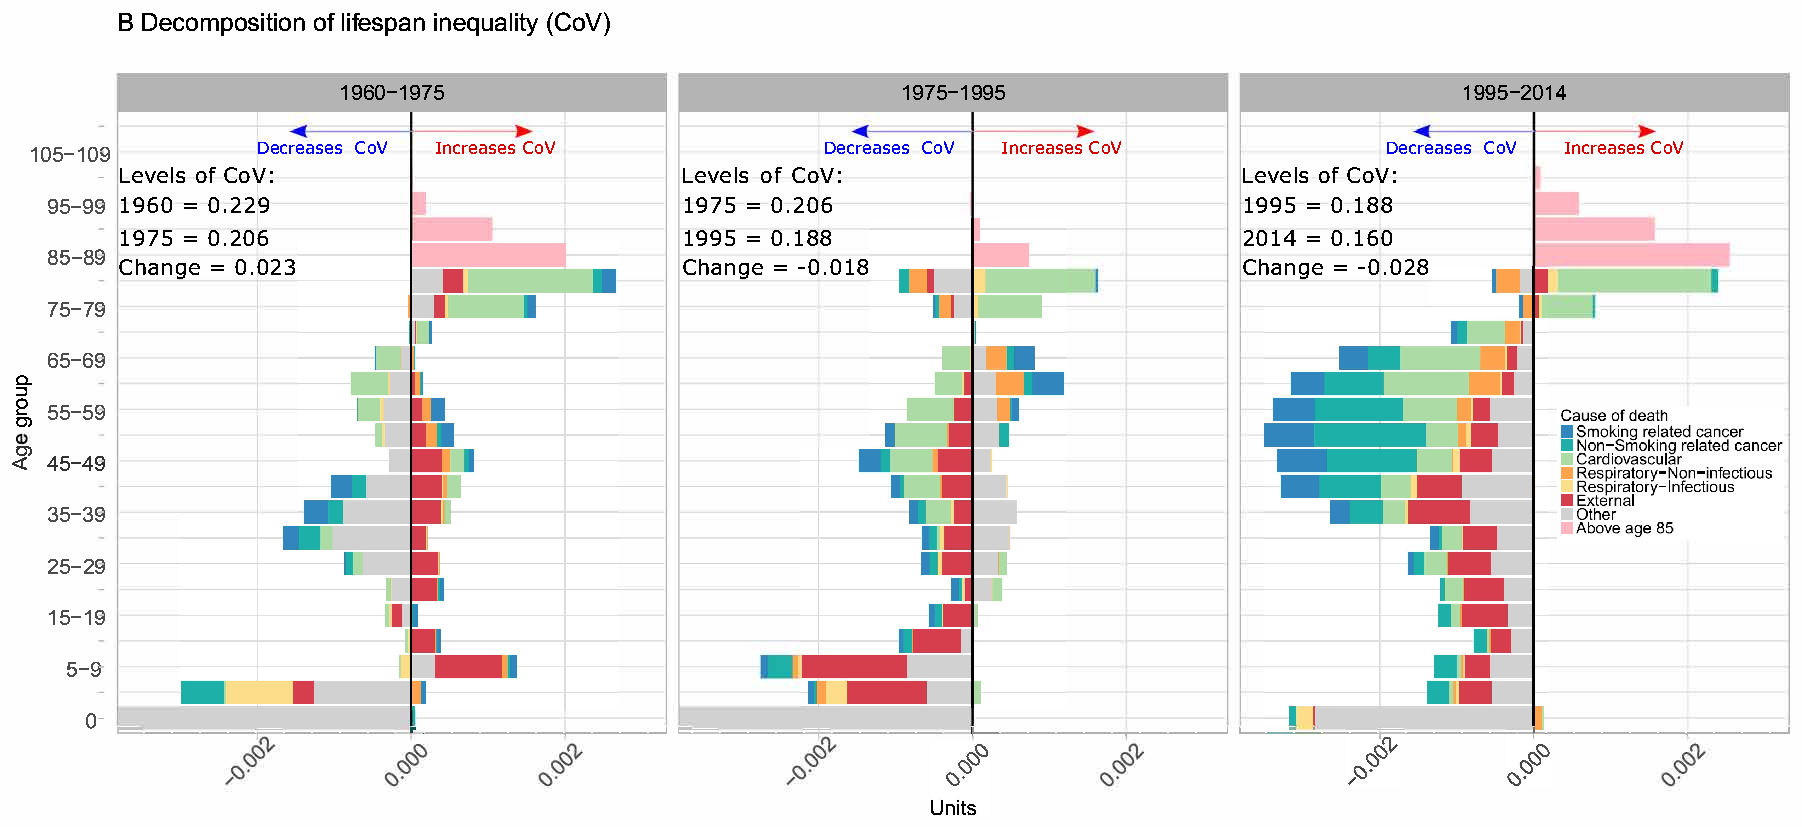
\includegraphics[scale=.41]{Figures/Figure_2_2}	
\end{frame}


\begin{frame}

\begin{center}
\hspace*{-.4in}
	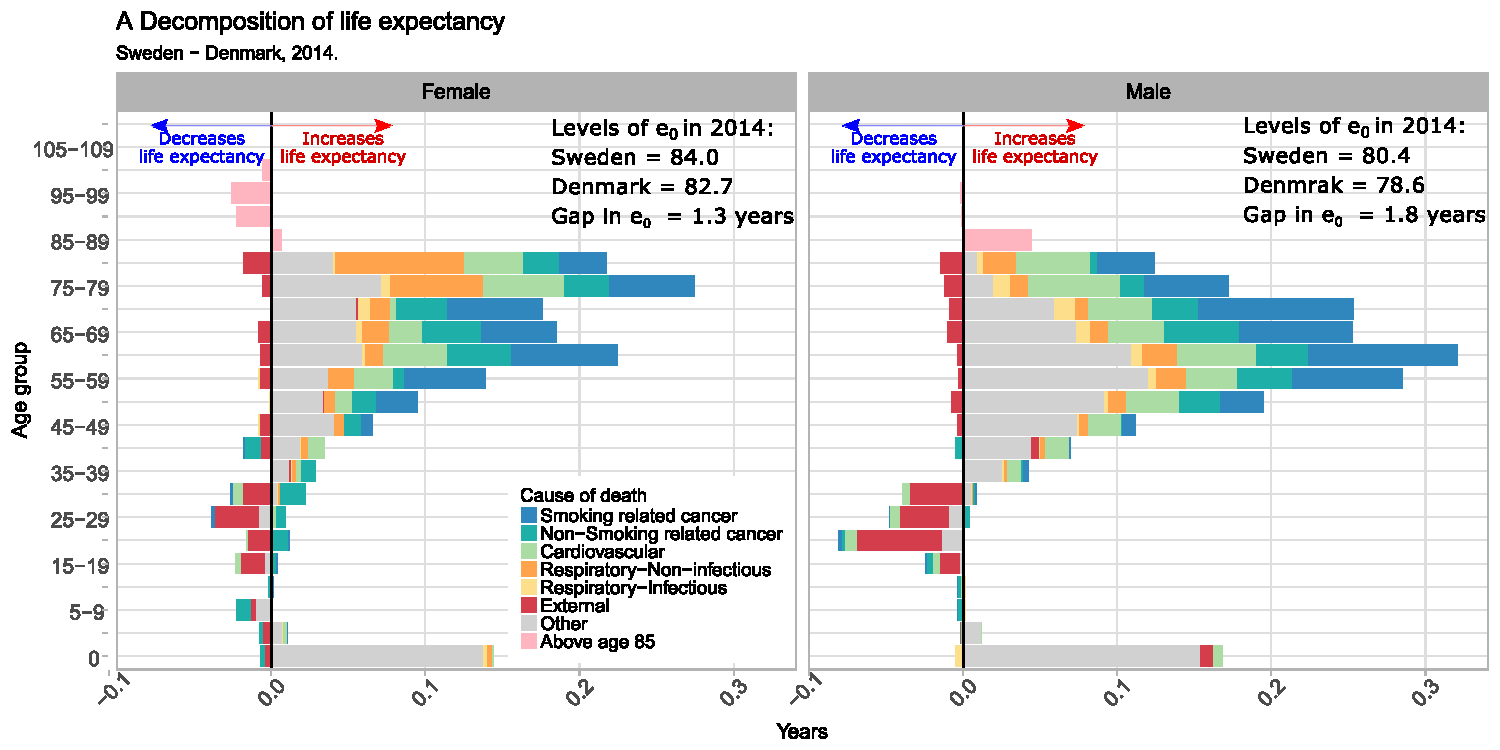
\includegraphics[scale=.5]{Figures/Figure_3_1}	
	\end{center}

\end{frame}

\begin{frame}
\begin{center}
\hspace*{-.4in}
	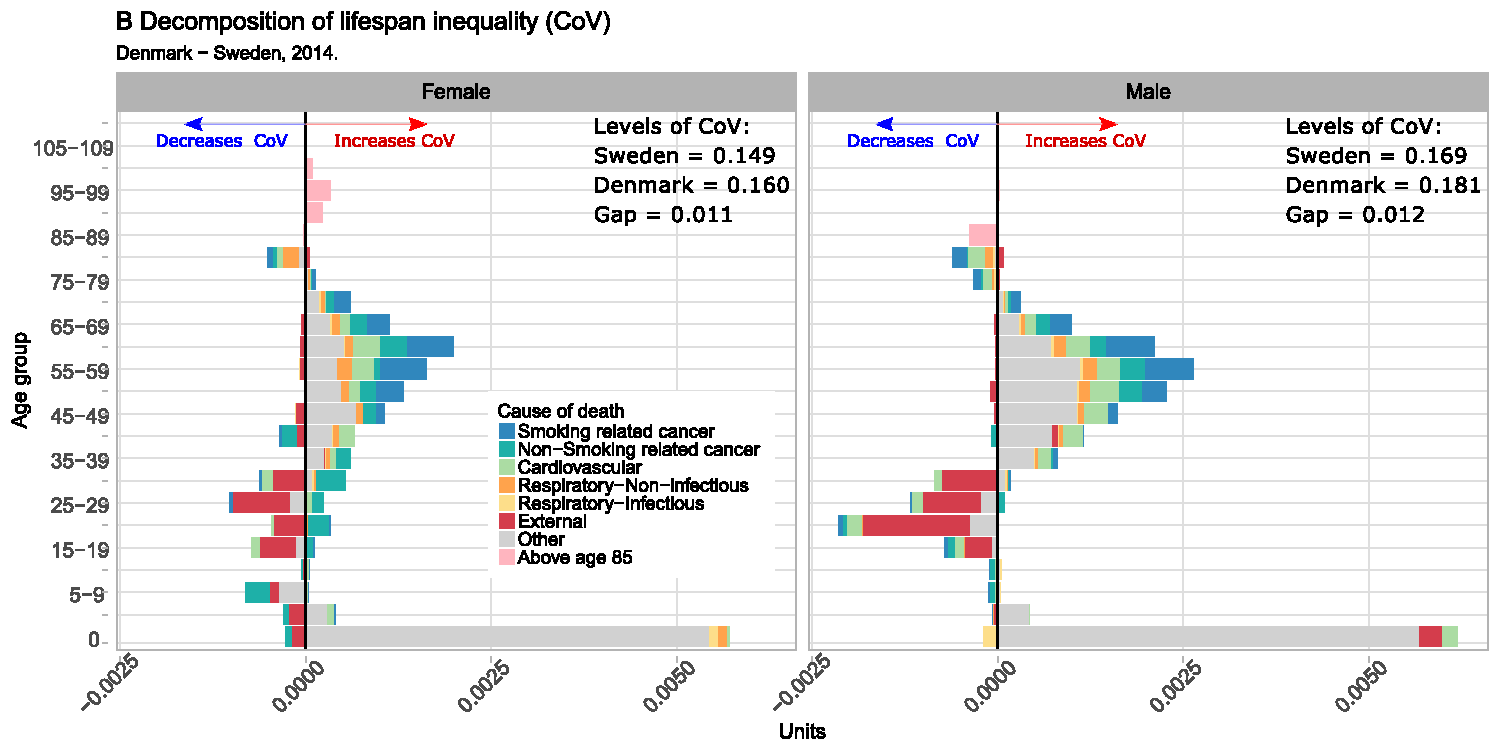
\includegraphics[scale=.5]{Figures/Figure_3_2}	
	\end{center}

\end{frame}

\begin{frame}
\begin{center}
	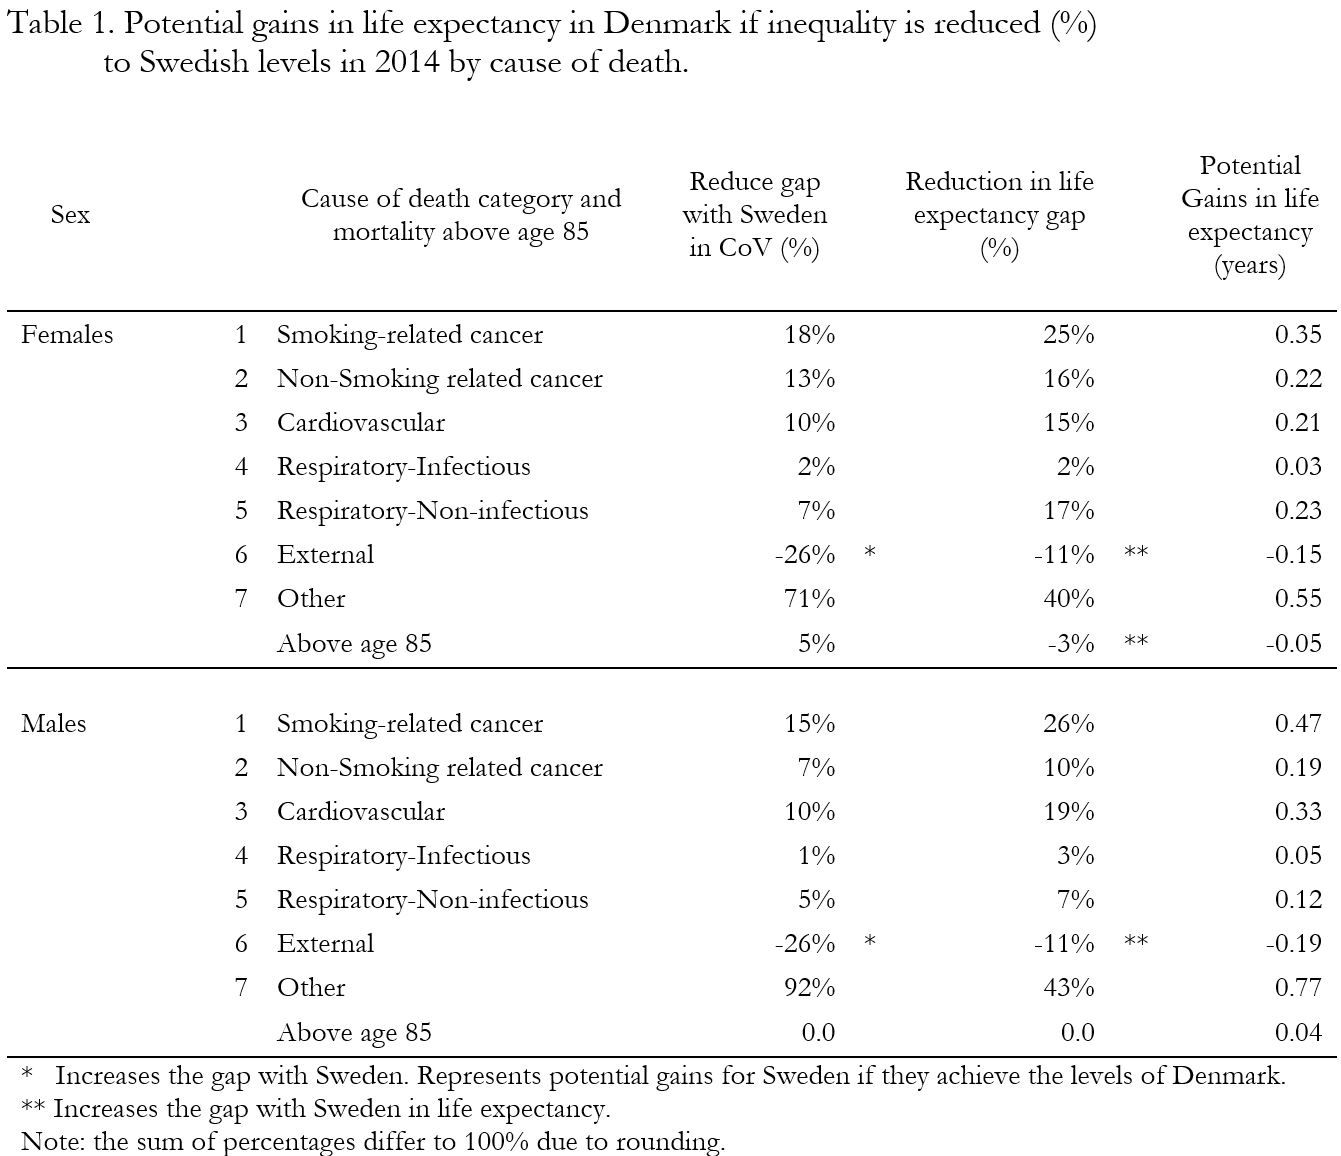
\includegraphics[scale=.26]{Figures/Table_1}	
	\end{center}

\end{frame}


\begin{frame}
\Large{\textbf{Key messages} \pause
		\begin{itemize}
		
		\item<1-> \textbf{Lifespan inequality} reflects $\longrightarrow$ 
		\begin{enumerate}
				 \item \textbf{heterogeneity} in ages at death.
				 \item \textbf{uncertainty} in the timing of death. 
		\end{enumerate}

		
		\item<3-> \textbf{Cancer mortality} $\longrightarrow$ biggest contributor to Danish-Swedish \textbf{life expectancy difference}.
		
		\item<4-> \textbf{Infant mortality} $\longrightarrow$ contributor to the 2014 Danish-Swedish \textbf{lifespan inequality difference}.
				
        \item<5-> \textbf{Denmark} can $\downarrow$ inequality in lifespans and $\uparrow$ life expectancy through a consistent policy target: \textbf{reducing cancer and infant mortality}.
		
		\end{itemize}
		
}

\end{frame}


%%%%%%%%%%%%%%%%%%%%%%%%%%%%%%%%%%%%%%%%%%%%%%%%%%%%%%%%%%%%%%%%%%%%%%%%

%%%%%%%%%%%%%%%%%%%%%%%%%%%%%%%%%%%%%%%%%%%%%%%%%%%%%%%%%%%%%%%%%%%%%%%%
\begin{frame}
 \begin{center}
	\begin{center}
	 \textbf{Potential gains in Denmark: Cancer and Infant Mortality}
	\end{center}
	
	\bigskip
	\bigskip
More information: 

Email: jmaburto@health.sdu.dk 

\faTwitter \quad  @jm\_aburto 

\faGithub \quad @jmaburto 

Shinnyapp: \url{https://jmaburto.shinyapps.io/DK_App/}


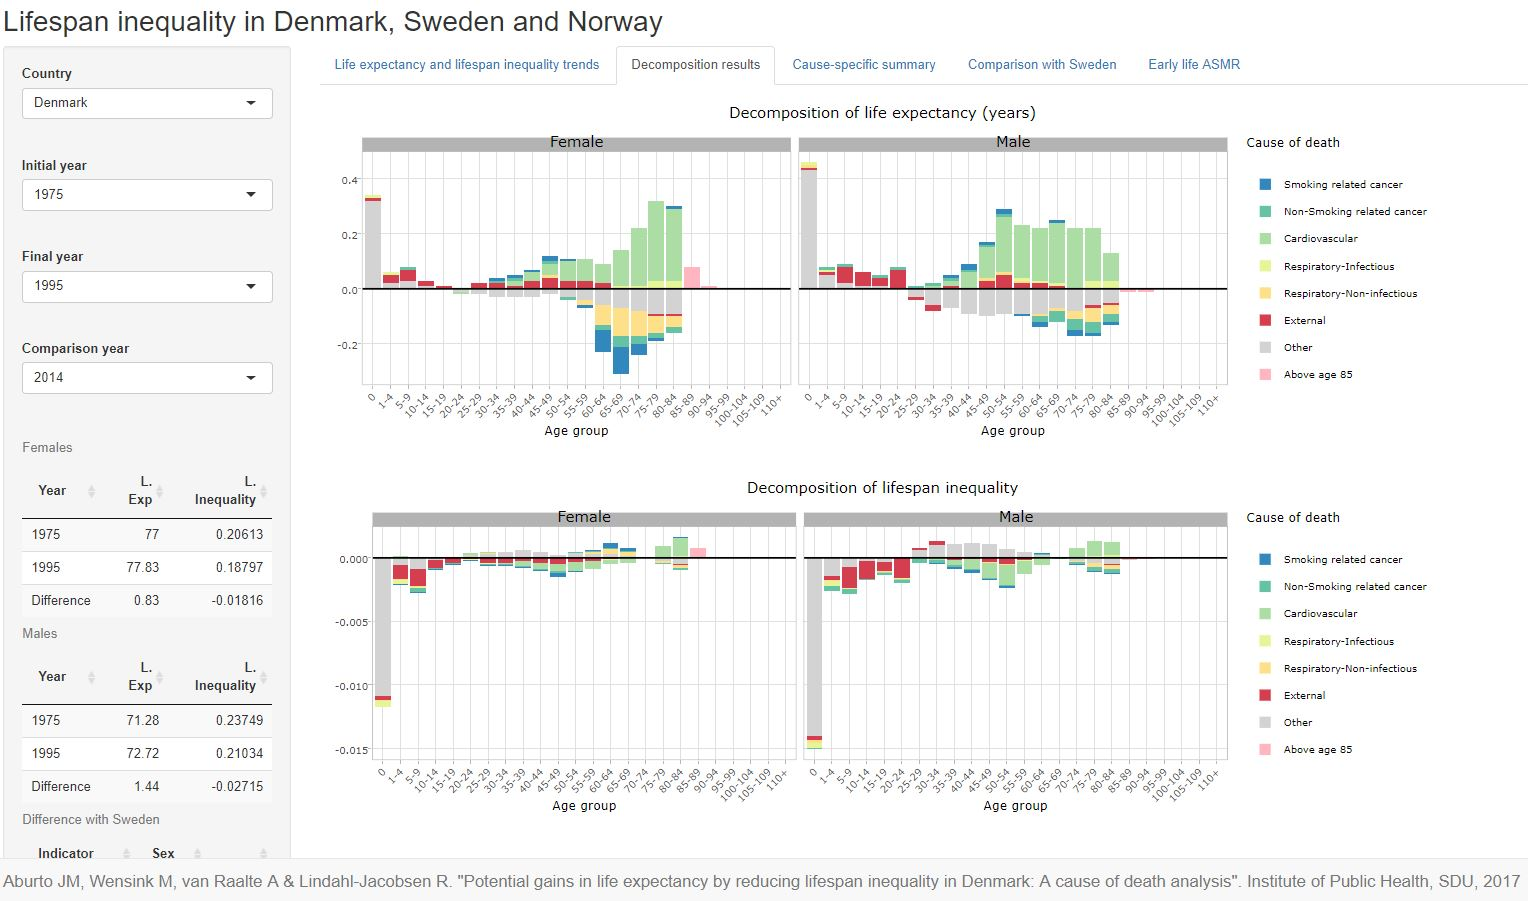
\includegraphics[scale=0.25]{Figures/ShinyappDK} \\   

\end{center}

\end{frame}




\end{document}
	

